\documentclass[10pt]{article}
\usepackage{icmlko}

\icmlmeta{IP 파운데이션 월드모델}{272}{안쪽 둘이 다른 답을 낸다}{F18 깊이를 재니 안쪽 두 방식이 3 과 5 를 짚고 유보는 봉우리가 아예 없다 --- 손잡이가 하나 더 죽었다}

\begin{document}

\twocolumn[
\icmlheader

\begin{abstract}
챔피언이 F18 로 돌아왔는데(노트 268) 그 초매개변수는 축이 다섯이던 시절에
정해진 것이다 --- 깊이 4 · 220회 · lr 0.06 · 배깅 8. 축이 스물셋이 된 지금
깊이가 안 맞을 수 있다. 깊이 2$\sim$6 을 \textbf{안쪽 두 방식}과 유보로 다
쟀다. \textbf{안쪽 둘이 다른 답을 낸다}: 실험실 기본인 7:3 분할
(\texttt{tune.inner\_split})은 \textbf{깊이 3}을 짚고(0.5250 · \textbf{0.5268} ·
0.5264 · 0.5228 · 0.5201), 노트 244가 권한 경계 앞 한 조각(2024)은
\textbf{깊이 5}를 짚는다(0.4808 · 0.4848 · 0.4868 · \textbf{0.4885} · 0.4830).
\textbf{둘 다 실험실 규약에서 떨어진다} --- 봉우리 지수가 0.269 와 0.481 로
문턱 0.5 를 못 넘고 단조도 0.700 · 0.400 으로 0.8 아래다
(\texttt{tune.accept} 가 둘 다 \texttt{False}). 유보는 또 다르다 ---
\textbf{봉우리가 아예 없다.} 0.4629 $\to$ 0.4754 $\to$ 0.4845 $\to$ 0.4857
$\to$ 0.4863 으로 끝까지 오르는데 증분이 $+$0.0125 $\to$ $+$0.0091 $\to$
$+$0.0012 $\to$ $+$0.0006 으로 깊이 4 에서 이미 포화한다. 깊이 4 에서 6 까지
전부 합쳐 $+$0.0018 --- 노트 245의 0.010 선 5분의 1이다. \textbf{깊이 4 를
그대로 둔다.} 안쪽으로 못 정하고(규약이 거부) 유보로도 못 정한다(선 아래).
노트 216이 알파와 $\tau$ 에서, 노트 243이 $\tau$ 에서 본 것과 같은 결말이다
--- \textbf{이 판에서 조율 손잡이는 세 번째로 죽었다.}
\end{abstract}
]

\section{왜 다시 재나}

노트 268이 챔피언을 F23 에서 F18 로 되돌렸다. 그런데 F18 의 손잡이는
\texttt{depth=4, it=220, lr=0.06, K=8} 로 노트 145 언저리에 정해진 것이고,
그때 판은 축이 다섯이었다. 지금은 스물셋이다. \textbf{축이 네 배 늘었는데
깊이가 그대로일 이유가 없다.}

깊이는 안쪽으로 정할 수 있는 종류다 --- 라벨을 안 보고 학습 구간만 갈라
고르면 된다. \texttt{lab/tune.py} 가 그러라고 있는 자리다.

\section{안쪽 둘이 다른 답을 낸다}

두 방식으로 쟀다. 실험실 기본인 \texttt{tune.inner\_split}(도메인마다 연도
70분위로 7:3)과 노트 244가 권한 \textbf{경계 앞 한 조각}(2024년만 평가).

\begin{center}\small
\begin{tabular}{lrrrrr}
\hline
깊이 & 2 & 3 & 4 & 5 & 6 \\
\hline
안쪽 7:3 & 0.5250 & \textbf{0.5268} & 0.5264 & 0.5228 & 0.5201 \\
안쪽 2024 & 0.4808 & 0.4848 & 0.4868 & \textbf{0.4885} & 0.4830 \\
유보 & 0.4629 & 0.4754 & 0.4845 & 0.4857 & \textbf{0.4863} \\
\hline
\end{tabular}
\end{center}

\textbf{7:3 은 3 을, 2024 조각은 5 를 짚는다.} 같은 자료 · 같은 격자인데
자르는 곳이 다르다는 것만으로 답이 두 칸 옮겨 간다.

\begin{figure}[t]
\centering
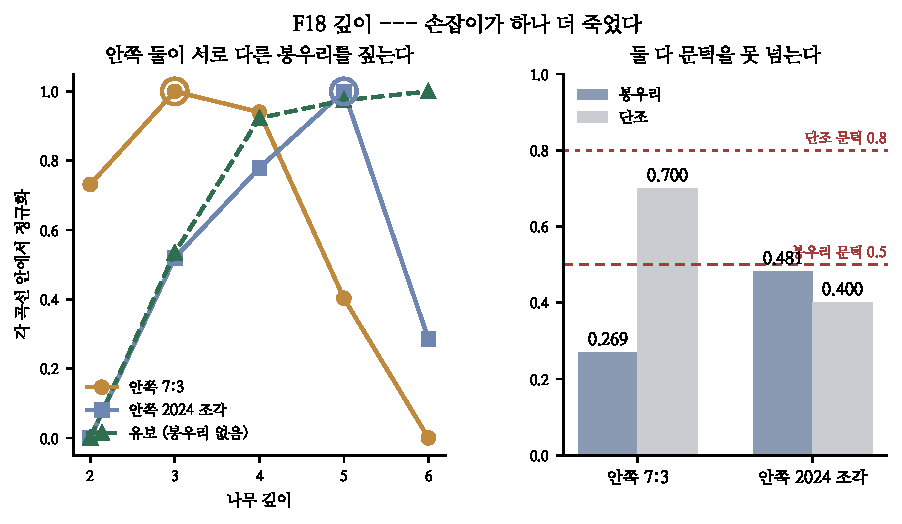
\includegraphics[width=\columnwidth]{figs/depth.pdf}
\caption{왼쪽 --- 곡선마다 제 안에서 정규화(동그라미가 각자의 봉우리).
오른쪽 --- 실험실 규약의 두 지수.}
\end{figure}

\section{둘 다 규약에서 떨어진다}

노트 190 · 216이 세운 조항은 ``곡면이 평평하면 안 고른다''이다 --- 봉우리
지수 $\ge 0.5$ 이거나 단조 지수 $\ge 0.8$ 이라야 한다.

\begin{center}\small
\begin{tabular}{lrrl}
\hline
 & 봉우리 & 단조 & \texttt{accept} \\
\hline
안쪽 7:3 & 0.269 & 0.700 & \textbf{False} \\
안쪽 2024 조각 & 0.481 & 0.400 & \textbf{False} \\
\hline
\end{tabular}
\end{center}

둘 다 못 넘는다. 2024 조각의 0.481 은 문턱에 바짝 붙었지만 넘지는 못했고,
넘었더라도 \texttt{tune.stable}(분할 다섯을 옮겨 최고가 그대로인지)이 남아
있었다.

\textbf{규약이 옳게 작동했다.} 7:3 곡선의 폭은 0.0067 이고 위 셋
(3 · 4 · 2)이 0.0018 안에 모여 있다 --- 봉우리라고 부를 것이 아니다. 규약이
없었으면 ``안쪽이 3 을 골랐다''고 적고 깊이를 내렸을 것이다.

\section{유보는 봉우리가 없다}

정작 유보는 \textbf{끝까지 오른다.} 그런데 증분을 보면 이야기가 끝난다.

\begin{center}\small
\begin{tabular}{lrrrr}
\hline
깊이 & 2$\to$3 & 3$\to$4 & 4$\to$5 & 5$\to$6 \\
\hline
증분 & $+$0.0125 & $+$0.0091 & $+$0.0012 & $+$0.0006 \\
\hline
\end{tabular}
\end{center}

\textbf{깊이 4 에서 이미 포화한다.} 4 에서 6 까지 다 합쳐 $+$0.0018 이고,
그것은 노트 245가 그은 0.010 선의 5분의 1이다. 그 자리는 안쪽 신뢰도가
0.34 이고(노트 244) 유보로 정하면 엿보기다(노트 245).

\textbf{깊이 4 를 그대로 둔다.} 얻을 것이 $+$0.0018 인데 근거가 없다.

\section{세 번째로 죽은 손잡이}

\begin{center}\small
\begin{tabular}{lll}
\hline
노트 & 손잡이 & 결말 \\
\hline
216 & 능형 알파 & 봉우리 0.63 통과, 바깥 이득 $-$0.0002 \\
216 · 243 & 감쇠 $\tau$ & 안정 2/5 로 막힘, 17축에선 0/13 \\
\textbf{272} & \textbf{나무 깊이} & \textbf{봉우리 0.27 · 0.48 로 거부} \\
\hline
\end{tabular}
\end{center}

\textbf{이 판에서 조율 손잡이가 산 적이 한 번도 없다.} 노트 190이 ``능형은
봉우리 0.81 로 $+$0.011$\sim$0.013 을 얻는다''고 적었는데 그것은 축이
다섯이던 시절이다. 축이 늘면서 곡면이 평평해졌다.

읽는 법이 하나 붙는다. \textbf{손잡이가 죽었다는 것은 모형이 나쁘다는 뜻이
아니라 그 축들이 깊이를 별로 안 탄다는 뜻이다.} 깊이 2 에서 6 까지 유보가
0.4629 에서 0.4863 으로 움직이는데, 그 폭 0.023 은 노트 260이 축 둘을
더해서 얻은 것($+$0.0224)과 비슷하다. \textbf{같은 값을 손잡이로도 얻을 수
있지만 근거를 못 만든다.}

\paragraph{남은 것}
\begin{center}\small
\begin{tabular}{ll}
\hline
갈래 & 왜 \\
\hline
안쪽 둘의 불일치 & 어느 자르기가 옳은가는 아직 모른다 \\
다른 손잡이 & \texttt{it} · \texttt{lr} · \texttt{K} 는 안 봤다 \\
웹툰 시계 몫 0.77 & 몫 27\% 라 판에 제일 크게 실린다 \\
포화 지점 & 깊이 4 가 포화면 다른 축 집합에서도 그런가 \\
\hline
\end{tabular}
\end{center}

\paragraph{규약} 손잡이를 재면 \textbf{안쪽을 두 가지로 잘라 본다.} 하나만
쓰면 ``안쪽이 골랐다''가 자르는 자리의 우연일 수 있다 --- 여기서는 3 과 5 로
갈렸고, 둘 다 규약에서 떨어져 다행히 같은 결론이 됐다.

\end{document}
